
\begin{frame}{Bitcoin}
  \begin{block}{Overview}
    \begin{itemize}
      \item Decentralized digital currency.
      \item 2008, Satoshi Nakamoto.
      \item Peer-to-peer (no bank, central authority). 
      \item New block every 10 minutes.
      \item Wallet (digital credentials).
      \item Key pair, public and private key.
      \item Amount of coins is fixed, from the beginning.
      \item 2010: first real life payment -- pizza order, 10 000 bitcoins, worth \$30.
    \end{itemize}
  \end{block}
\end{frame}

\begin{frame}{Bitcoin}
  \begin{block}{Value}
    \begin{center}
      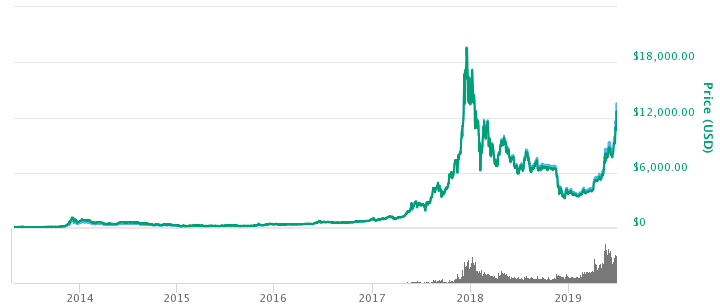
\includegraphics[height=4cm]{img/price.png}
    \end{center}
  \end{block}
  \begin{block}{Value}
    \begin{center}
      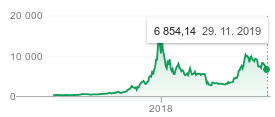
\includegraphics[height=2cm]{img/price-now.png}
    \end{center}
  \end{block}
\end{frame}


\begin{frame}{Bitcoin}
  \begin{block}{Mining 1/2}
    \begin{itemize}
      \item Running a PoW to accept a new block.
      \item Distributed timestamp.
      \item Identify a block that, when hashed twice with SHA-256, yields a number smaller than difficulty level.
      \item Verification is possible using one SHA-256 run.
      \item Increment a nonce until a value is found that gives the block's hash the required number of leading zeros.
      \item $https://emn178.github.io/online-tools/sha256.html$
    \end{itemize}
  \end{block}
\end{frame}

\begin{frame}{Bitcoin}
  \begin{block}{Mining 2/2}
    \begin{center}
      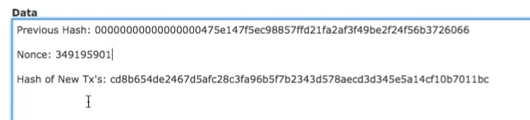
\includegraphics[height=2cm]{img/content.png}
    \end{center}
  \end{block}
\end{frame}

\begin{frame}{Ethereum}
  \begin{block}{Overview}
    \begin{itemize}
      \item 2013 Vitalik Buterin.
      \item Distributed open source blockchain based platform.
      \item Smart Contracts.
    \end{itemize}
  \end{block}
  \begin{block}{Ether}
    \begin{itemize}
      \item Cryptocurrency.
      \item Block time is 10-15s. 
      \item Mining generates new coins. 
      \item Different PoW (reduces benefits of specialized HW).
    \end{itemize}
  \end{block}
  \begin{block}{Smart contracts}
    \begin{itemize}
      \item Scripting functionality of Ethereum platform.
      \item Application development. 
      \item Language: combination of C, JavaScript, Python and Go. 
    \end{itemize}
  \end{block}
\end{frame}

